\documentclass[a4paper,10pt]{article}
\usepackage[utf8x]{inputenc}
\usepackage{graphicx}
\usepackage{pgf}
\pgfdeclareimage[height=1cm]{myimage}{p1_q1.png}
\usepackage{listings}


%opening   
\title{ \textbf{Universidade de Brasília - Campus Gama \\ 
        Orientação a objetos \\ Exercício de Programação }}
\date{}

\author{Paulo Meirelles}

\begin{document}
\maketitle

\paragraph{}
\textbf{Atenção:} Este é um exercíco de programação que visa a aplicação de 
  alguns conceitos de orientação a objetos aprendidos durante a disciplina de 
  orientação a objetos. Recomenda-se o trabalho contínuo em tal exercício, pois
  acredita-se que o mesmo dificilmente pode ser implementado em um ou dois dias
  com a devida qualidade exigida. Este exercíco busca avaliar os seguintes
  conceitos:

\begin{itemize}
 \item Criação de classes e objetos.
 \item Utilização de atributos, métodos e construtores. 
 \item Utilização de herança.
\end{itemize}

Para o melhor aproveitamento do aluno, recomenda-se que o mesmo busque várias
referências externas para auxiliar na resolução do exercíco.

\section{Introdução}

\paragraph{}
Nos últimos anos, o processamento de imagens digitais passou a chamar a atenção
de vários pesquisadores por dois motivos: aperfeiçoar a informação visual para
uma melhor interpretação humana e processamento de dados de cenas para
percepção automática através de imagens. Neste contexto, surgiu a
necessidade de se manipular imagens computacionalmente e de buscar técnicas
para lidar com as mesmas.

\paragraph{}
Uma imagem pode ser definida matematicamente como uma função bidimensional de
intensidade da luz definida por $f(x, y)$, onde $x$ e $y$ denotam as 
coordenadas espaciais e o valor de $f$ em qualquer ponto. $(x,y)$ é
proporcional ao brilho (níveis de cinza) da imagem naquele ponto. Com 
base nisto é possível considerar uma imagem como sendo uma matriz cujo as 
coordenadas indicam um ponto na imagem e o valor indica o nível de cinza 
naquele ponto.

\begin{figure}[ht]
 \center
 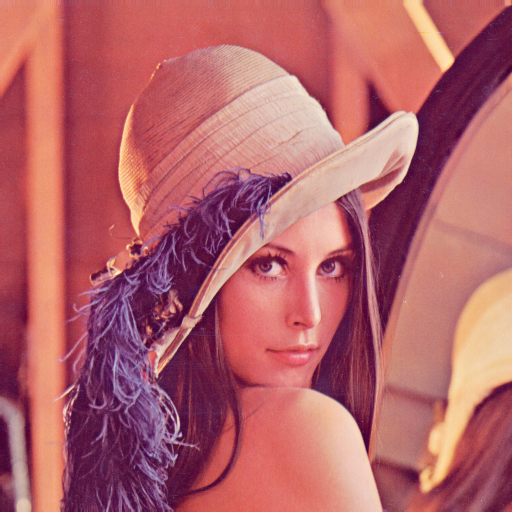
\includegraphics[width=5cm]{imagem/Lenna.png}
 \caption {Uma imagem é definida como: $f(x,y)$}
\end{figure}

\paragraph{}
Computacionalmente, uma imagem é representada como uma matriz. Contudo, devido
a questões de redução de tamanho essas imagens podem ser comprimidas em
formatos específicos como PNG, JPEG, BMP, etc. Tais formatos utilizam
algoritmos específicos de compressão e por isto apresentam um grau de
complexidade maior para serem manuseadas. Uma alternativa didática para
entender como as imagens comportam-se é o formato PGM (\textit{Portable
Graymap Format}). Este formato, pode ser manipulado como uma simples leitura
de arquivo seguida da correta interpretação dos seus campos. Veja abaixo a
estrutura deste tipo de imagem:

\begin{itemize}
  \item Número mágico (P5)
  \item Comentário (Começam com \#)
  \item Dimensões (Altura e largura)
  \item Nível máximo de cinza
  \item Pixels
\end{itemize}

\paragraph{}
Sabendo que uma imagem pode ser tratada como uma matriz é possível realizar a 
aplicação de máscaras espaciais (também conhecidas como filtros espaciais),
estas consistem de matrizes 3x3, 5x5, 7x7, etc. 

\begin{figure}[ht]
 \center
 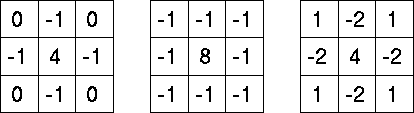
\includegraphics[width=10cm]{imagem/lapmasks2.png}
 \caption {Exemplos de filtros}
\end{figure}

Estas máscaras, são aplicadas sobre cada pixel de uma imagem. Normalmente tais
máscaras são definidas em números ímpares para que tenha um meio, isto é
importante devido ao fato de que a aplicação do filtro consiste em somar os
produtos entre os coeficientes da máscara e as intensidades de pixels sob a
máscara numa posição específica da imagem. Matemáticamente, supondo que temos
o filtro composto pelos elementos $w$ e uma imagem cujo os elementos são
definidos por $z$, tem-se:

$$R = w_1z_1 + w_2z_2 + ... + w_xz_x$$

Em posse de tais informações é possível aplicar um grande número de operações
sobre a imagem. Alguns tipos mais simples como a aplicação de um negativo e 
outros mais complexos como a aplicação de filtros.

\paragraph{}
Um dos filtros mais comuns de aplicação são os chamados filtros de suavização.
Estes filtros podem ser utilizados para borrar a imagem e reduzir ruídos. 
A principal aplicação deste tipo de filtro, consiste na remoção de
pequenas imperfeições antes de aplicar algum outro filtro. Veja abaixo a
máscara:

\begin{figure}[ht]
 \center
 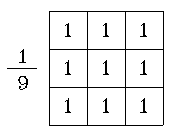
\includegraphics[width=3cm]{imagem/passa_baixa.png}
 \caption {Filtro de suavização passa-baixa}
\end{figure}

Outro filtro muito comum é o \textit{sharpen}, veja abaixo como é a matriz que
representa tal filtro:

\begin{figure}[ht]
 \center
 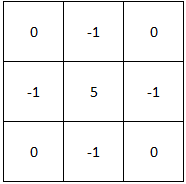
\includegraphics[width=3cm]{imagem/sharpen.png}
 \caption {Sharpen}
\end{figure}

\section{Exercício}

\subsection{Objetivos gerais do exercício}
\paragraph{}
O princípal objetivo deste exercício é aplicar os seguintes conceitos de 
orientação a objetos:

\begin{itemize}
  \item Classes.
  \item Atributos.
  \item Métodos.
  \item Construtores.
  \item Herança.
\end{itemize}

Você poderá encontrar o algoritmo das funções de leitura e aplicação de filtros
na seção Algoritmos. Adicionalmente, é possível verificar algumas dicas ao
final deste arquivo.

\subsection{Fase Zero: Preparação}

Visando manter a mesma estrutura dos projetos, crie a seguinte estrutura de
pastas:

\begin{itemize}
  \item bin: Pasta onde será mantido o binário.
  \item include: Pasta que manterá os \textit{headers}.
  \item source: Pasta que manterá as implementações dos \textit{hearders}.
  \item obj: Pasta que receberá os arquivos objetos.
  \item doc: Pasta onde conterá qualquer informação extra de documentação.
\end{itemize}

\paragraph{}
Por fim, crie os seguintes arquivos:

\begin{itemize}
  \item Makefile: Crie o arquivo Makefile que compilará o seu código e
    salvará o arquivo compilado na pasta bin.
  \item README.md: Explique de forma ORGANIZADA e direta como compilar e
    executar o seu programa.
\end{itemize}

Extra:

\begin{itemize}
  \item Doxygen: Crie o arquivo Doxygen e documente o seu código utilizando
    tal ferramenta.
  \item test: Crie a pasta "test" e implemente testes unitários para o seu
    código.
\end{itemize}

\subsection{Primeira fase: Trabalhando com a imagem}

A primeira parte do exercício consiste em criar um programa em C++ que
manipule uma imagem do tipo PGM. O seu programa deve realizar no mínimo as
seguintes tarefas:

\begin{enumerate}
  \item Leia uma imagem PGM, recebendo o caminho da imagem.
  \item Crie um método que permita salvar a imagem em outro local com outro
    nome.
\end{enumerate}

Espera-se a implementação de pelo menos uma classe contendo atributos para
manter os dados da imagem e métodos para manipular tais dados.

\subsection{Segunda fase: Trabalhando com filtros}

Após ler e armazernar os dados referêntes as imagem, crie uma maneira de 
aplicar as seguintes transformações:

\begin{enumerate}
  \item Negativo.
  \item Smooth.
  \item Sharpen.
\end{enumerate}

Lembre-se que o seu objetivo é utilizar os conceitos de Orientação a Objetos, 
logo recomenda-se uma reflecção buscando abstrair tais filtros. Espera-se pelo
menos uma classe geral e classes filhas que implementem os filtros.
\\
\textbf{DICA:} Crie uma classe pai para aplicar filtros e classes filhas
que apliquem filtros específicos.\\
\textbf{DICA:} Veja a seção de Algoritmos para ver como implementar os filtros
solicitados.

\newpage
\section{Algoritmos}

\paragraph{}
Como a implementação dos algoritmos não é o foco deste trabalho, segue o
diagrama e os trecho de código que seram necessários. Apesar do código está 
sendo fornecido, vale observar que é trabalho do estudante entender e adaptar 
os trechos de códigos.

\subsection{Leitura da imagem}

\paragraph{}
Algoritmo geral para a leitura da imagem PGM.

\begin{figure}[ht]
 \center
 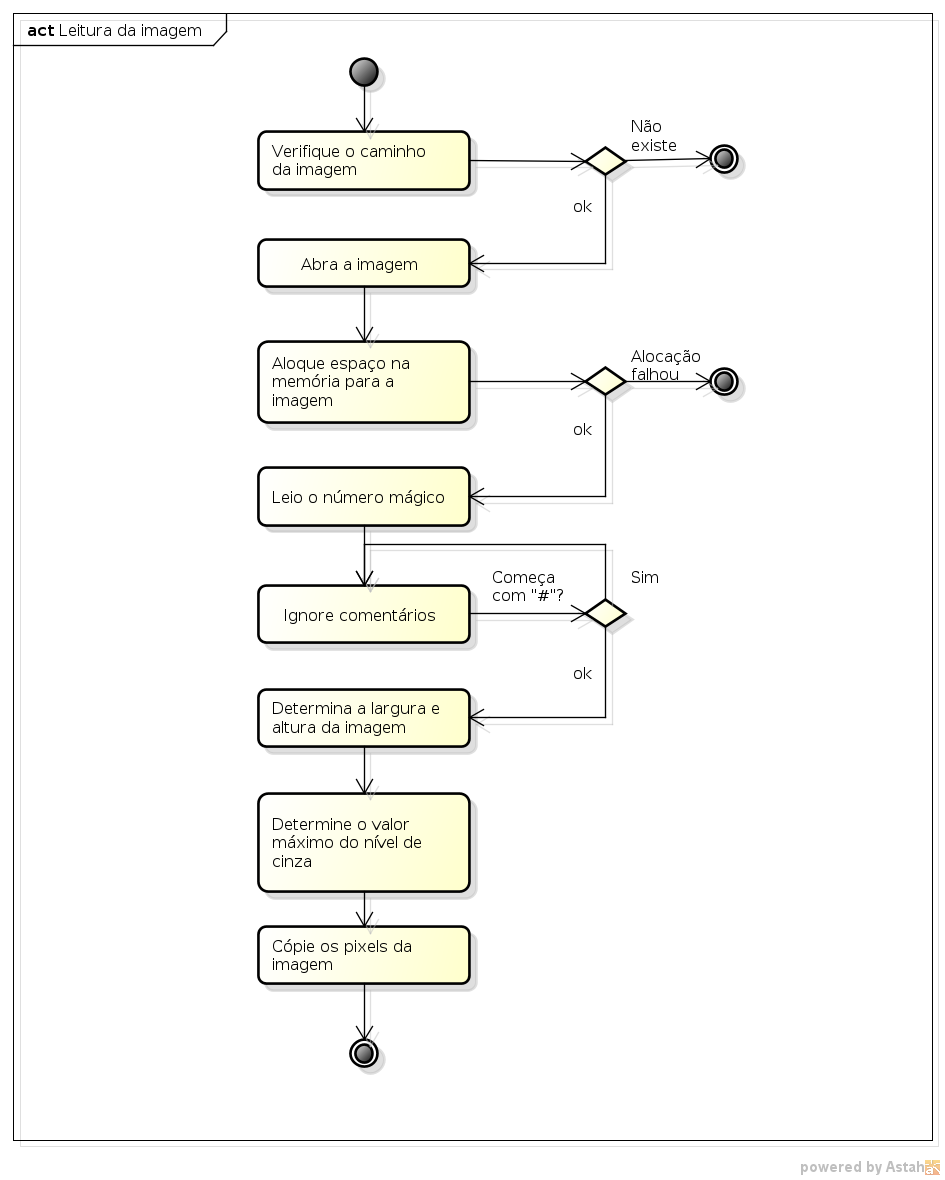
\includegraphics[width=10cm]{imagem/Leitura_da_imagem.png}
\end{figure}

\subsection{Aplicar o negativo}

\paragraph{}
Para aplicar o negativo, basta realizar uma simples subtração pixel a pixel.
Veja o trecho de código abaixo:

\begin{lstlisting}
...
for (i = 0; i < image->width * image->height; i++)
	copy->pixels[i] = image->max_level - image->pixels[i];
...
\end{lstlisting}

\subsection{Aplicar filtro}

\paragraph{}
O processo de aplicar filtros é o mesmo para o \textit{smooth} e para o 
\textit{sharpen}. Neste contexto, análise o loop abaixo (lembre-se que o 
mesmo percorre toda a imagem aplicando um filtro pixel a pixel):

\begin{lstlisting}

for (i = limit; i < image->w - limit; i++)
{
	for (j = limit; j < image->h - limit; j++)
	{
		value = 0;
		for (x = -1; x <= 1; x++)
		{
			for (y = -1; y <= 1; y++)
			{
				value += filter[(x+1) + 
				  size*(y+1)]*image->pixels[(i + x) + 
				  (y + j)*image->w];
			}
		}

		value /= div;

		value = value < 0 ? 0 : value;
		value = value > 255 ? 255 : value;

		copy->pixels[i + j*image->w] = value;
	}
}

\end{lstlisting}

\subsection{Aplicar smooth}

\paragraph{}
Como visto na seção introdutária, segue o filtro de suavização:

\begin{lstlisting}

int filter[] = {1, 1, 1, 1, 1, 1, 1, 1, 1};

\end{lstlisting}

\subsection{Aplicar sharpen}

\paragraph{}
Veja o filtro \textit{sharpen}:

\begin{lstlisting}

filter[] = {0, -1, 0, -1, 5, -1, 0, -1, 0};

\end{lstlisting}


\section{Referências}

\paragraph{}
Grande parte desta fundamentação teórica, foi baseada nas referências abaixo:

\begin{itemize}
  \item Processamento de Imagens digitais, Rafel C. Gonzalez, Richard D. Woods.
  \item Laboratório 0 do curso de estrutura de dados da FGA, ministrado pelo 
	professor Edson Alves.
\end{itemize}

\end{document}
